\documentclass[nobib]{MSword}
% Class options:
%-------------------------------
% nobib         - skip bibliography code/ don't include bib
% math          - include math packages and useful math commands
% hidelinks     - hide hyperref colored link boxes
% wordlinks     - link color scheme similar to word


% Preamble code:
%%%%%%%%%%%%%%%%%%%%%%%%%%%%%%%%%%%%%%%%
\usepackage[english]{babel}
\usepackage{csquotes}
\usepackage{lipsum}

% % Uncomment using "Ctrl + /" (/ on numpad):
% % Customizing headers and footers:
% \fancypagestyle{custom}{%
%     \fancyhf{}% clears the footer and header
%     % Header:
%     \fancyhead[L]{}
%     \fancyhead[C]{}
%     \fancyhead[R]{}
%     % Footer:
%     \fancyfoot[L]{}
%     \fancyfoot[C]{}
%     \fancyfoot[R]{}
%         % Tips:
%         % ----
%         % L: left, C: center, R: right
%         % O: odd pages, E: even pages
%         % ----
%         % Example: \fancyghead[LO,RE]{Text}
%         % will produce "Text" left in the header
%         % on odd pages and right in the header on even pages.
%     % Rules/ lines:
%     \renewcommand{\headrulewidth}{0.4pt}
%     \renewcommand{\footrulewidth}{2pt}
% }
% % Changing the pagestyle:
% \pagestyle{custom}

%%%%%%%%%%%%%%%%%%%%%%%%%%%%%%%%%%%%%%%%

% Preamble information:
%%%%%%%%%%%%%%%%%%%%%%%%%%%%%%%%%%%%%%%%

\title{Frequency Response}
\author{Dre Mata}
\date{3 April 2023}

%%%%%%%%%%%%%%%%%%%%%%%%%%%%%%%%%%%%%%%%

% The document:
%%%%%%%%%%%%%%%%%%%%%%%%%%%%%%%%%%%%%%%%
\begin{document}

\maketitle
\begin{center}
    Part 1:
\end{center}
The objective of part 1 is to create a frequency response for the RLC circuit seen in the prelab. This will be shown by creating a Bode plots for the magnitude and angle. The first task of this was to create functions for the transfer function's magnitude and frequency response. After this was done plots for the transfer function's magnitude and angle were created. These plots can be seen in Figure one. The second task was to use scipy.signal.bode to plot the magnitude and frequency response of the transfer function. These plots can be seen in Figure two.

\begin{center}
    Part 2:
\end{center}
The objective of part 2 is to use the frequency response model developed as a filter for a multi-band input signal. The input signal is seen below.

$ x(t) = cos(2pi * 100t) + cos(2pi * 30243t) + sin(5pi * 500000t)$

The first task was to plot the input signal seen above. This can be seen in Figure three. The next task was to convert the input signal into the Z-domain using the scipy.signal.bilinear function. The next task was to use the scipy.signal.lfilter function to pass the input signal through the transfer function. The plot of the output signal can be seen in Figure three as well.


\begin{center}
    Questions:
\end{center}

1. Explain how the filter and filtered output in Part 2 makes sense given the Bode plots from Part 1. Discuss how the filter modifies specific frequencry bands, in Hz.

Just by looking at the bode plot of the magnitude for the transfer function I see that there is no way for the signal to be amplified so it makes sense that the output signal is in a range of (-1,1). 

2. Discuss the purpose and workings of scripy.signal.bilinear() and scipy. signal.lfilter().

The purpose of scripy.signal,bilinear is to transform the transfer function into the Z domain. The purpose of scipy.signal.lfilter is to run the input signal through the transfer function. The workings for both of these is that they take a numerator and a denominator for the transfer function. The bilinear then takes a sample frequency and the lfilter takes an input signal.

3. What happens if you use a different sampling frequency in scripy.signal.bilinear() than you used for the time-domain signal?

The graph could come out screwed or with low resolution.

\begin{center}
    Figures
\end{center}

Figure 1:

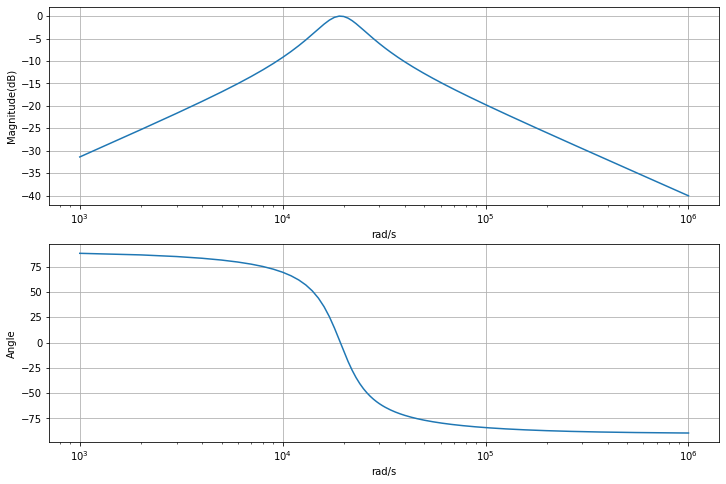
\includegraphics[scale = 0.6]
{txt/Lab10Fig1.png}

Figure 2:

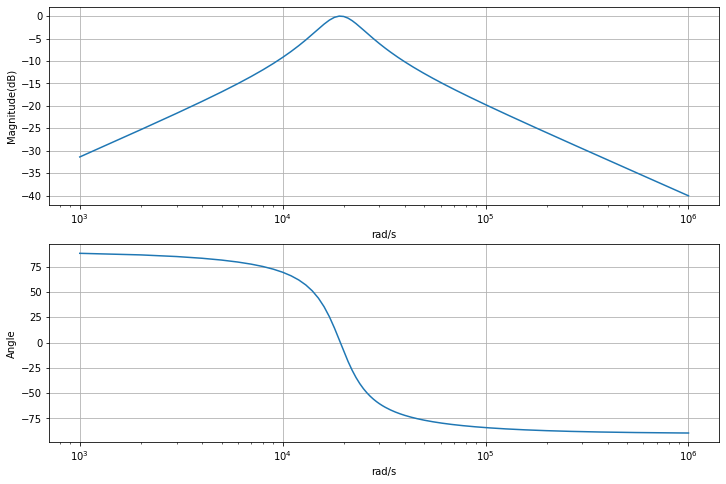
\includegraphics[scale = 0.6]
{txt/Lab10Fig2.png}


Figure 3:

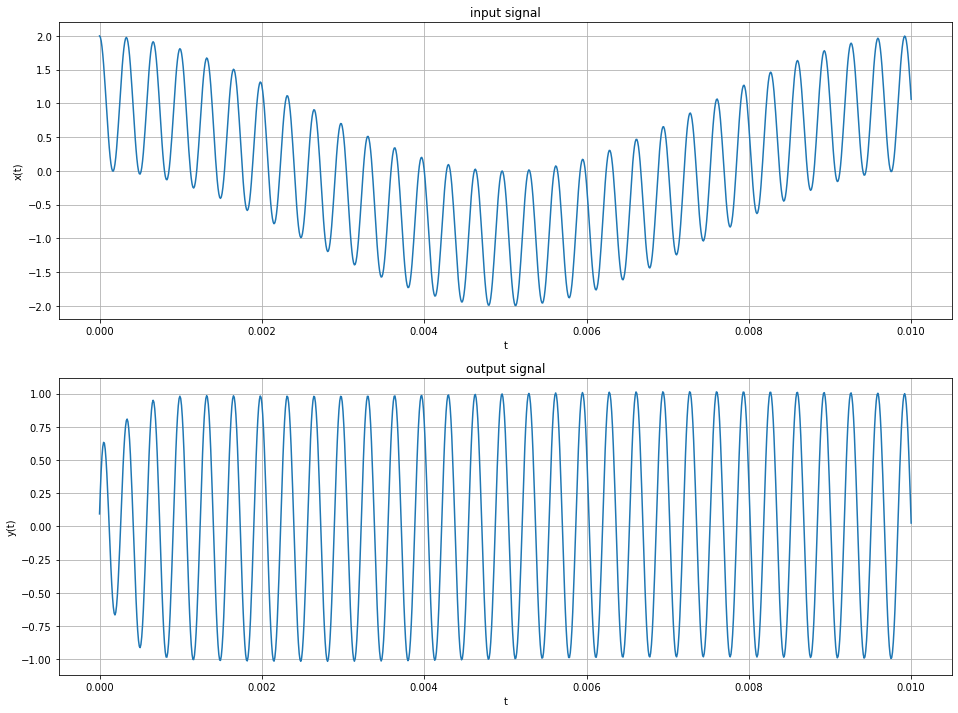
\includegraphics[scale = 0.45]
{txt/Lab10Fig4.png}

\begin{center}
    Conclusion
\end{center}
   This lab helped me gain a better understanding of how to use the frequency response tools and Bode plots in python. It was insight full to take the input signal and run it through the transfer function on python and also do it by hand to see how the signal would come out. After seeing they came out to be very close it helped me gain confidence in the software sig.lfitler.

\end{document}
%%%%%%%%%%%%%%%%%%%%%%%%%%%%%%%%%%%%%%%%

% Copyright Remarks:
%--------------------

% Copyright holder: Vebjørn S. Førde, copyright: CC BY 4.0
% Note: The author of this template is also the copyright holder.

% Below is an explanation of the CC BY 4.0. Additional statements/ 
% clarifications made by the author/copyright holder are marked with *.

% YOU ARE FREE TO:
% Share — copy and redistribute the material in any medium or format
% Adapt — remix, transform, and build upon the material
% for any purpose, even commercially.

% UNDER THE FOLLOWING TERMS:
% Attribution* — You must give appropriate credit, provide a link to the license,
% and indicate if changes were made. You may do so in any reasonable manner, but 
% not in any way that suggests the licensor endorses you or your use.

% *Note: 
% Attribution NOT NEEDED for: 
%       - PDF distibution (like sharing your PDF document)
%       - Use of (dummy)text and images provided in the template (obviously)
%       - Distributing parts of the template, and not the template as a whole
% I am not really concerned with being given credit. As long as you do not 
% claim to have made the template yourself in distributing it further, I have
% no complaints.

% No additional restrictions — You may not apply legal terms or technological 
% measures that legally restrict others from doing anything the license permits.

% NOTICES:
% No warranties are given.

% Disclaimer* (added by copyright holder):
% THE SOFTWARE IS PROVIDED "AS IS", WITHOUT WARRANTY OF ANY KIND, EXPRESS OR
% IMPLIED, INCLUDING BUT NOT LIMITED TO THE WARRANTIES OF MERCHANTABILITY,
% FITNESS FOR A PARTICULAR PURPOSE AND NONINFRINGEMENT. IN NO EVENT SHALL THE
% AUTHORS OR COPYRIGHT HOLDERS BE LIABLE FOR ANY CLAIM, DAMAGES OR OTHER
% LIABILITY, WHETHER IN AN ACTION OF CONTRACT, TORT OR OTHERWISE, ARISING FROM,
% OUT OF OR IN CONNECTION WITH THE SOFTWARE OR THE USE OR OTHER DEALINGS IN THE
% SOFTWARE.

% Read more about CC BY 4.0:
% https://creativecommons.org/licenses/by/4.0/